\documentclass{beamer}

\usepackage{graphicx}

\input{../../../../../texmacros/commands.tex}

\usetheme{Madrid}

\DeclareMathOperator{\RSS}{RSS}
\DeclareMathOperator*{\Argmin}{argmin}
\DeclareMathOperator*{\Argmax}{argmax}

\newcommand{\va}{\boldsymbol{a}}
\newcommand{\vb}{\boldsymbol{b}}
\renewcommand{\vx}{\boldsymbol{x}}
\renewcommand{\vy}{\boldsymbol{y}}
\newcommand{\vz}{\boldsymbol{z}}
\newcommand{\vW}{\boldsymbol{W}}
\newcommand{\lra}{\longrightarrow}

\begin{document}
    
\setlength{\parskip}{1em}
\begin{frame}
    \title{Neural Networks, Tensorflow, and Keras}
    \date{DATA 607 --- Session 7 --- 18/03/2019}
    \maketitle
\end{frame}

\begin{frame}{}
    Perceptron and logistic regression classifiers have linear decision boundaries.
    \begin{figure}
    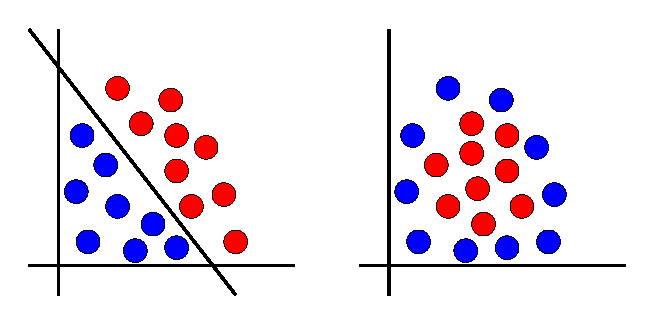
\includegraphics[]{linear/linear.pdf}
    \caption{Linearly separable, not linearly separable}
    \end{figure}
\end{frame}

\begin{frame}{}
    Perceptron, logistic regression \textbf{can} learn:
    \[
        f:\big\{(0, 0), (1, 0), (1, 1), (0, 1)\big\}\longrightarrow
        \{0,1\}
    \]
    \[
        f(0, 0) =  1,\quad f(1, 0) = f(1, 1) = f(0, 1) = 0
    \]

    \begin{figure}
        \only<1>{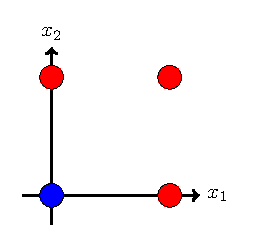
\includegraphics[]{one_and_three/one_and_three.pdf}}
        \only<2>{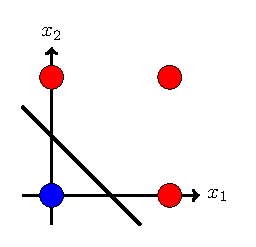
\includegraphics[]{one_and_three/one_and_three_2.pdf}}
        \caption{Graph of $f$}
    \end{figure}
\end{frame}

\begin{frame}{}
    \begin{figure}
        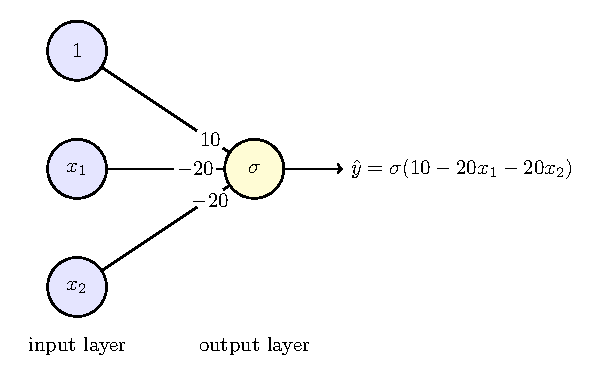
\includegraphics[scale=0.8]{one_and_three_nn/one_and_three_nn.pdf}
    \end{figure}

    \begin{center}
        \begin{tabular}{cc|c}
            $x_1$ & $x_2$ & $\widehat{y}$\\\hline
            $0$ & $0$ & $\sigma(10) \approx 1$\\
            $1$ & $0$ & $\sigma(-10) \approx 0$\\
            $0$ & $1$ & $\sigma(-10) \approx 0$\\
            $1$ & $1$ & $\sigma(-30) \approx 0$
        \end{tabular}
    \end{center}
\end{frame}

\begin{frame}{}
    Perceptron, logistic regression \textbf{can't} learn...
    \[
        f:\big\{(0, 0), (1, 0), (1, 1), (0, 1)\big\}\longrightarrow
        \{0,1\}
    \]
    \[
        f(0, 0) = f(1, 1) = 1,\quad f(1, 0) = f(0, 1) = 0
    \]

    \begin{figure}
        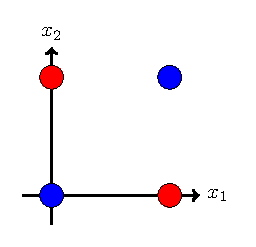
\includegraphics[]{two_and_two/two_and_two.pdf}
        \caption{Graph of $f$}
    \end{figure}
\end{frame}

\begin{frame}{}
    ... unless we introduce new features.
    \begin{figure}
        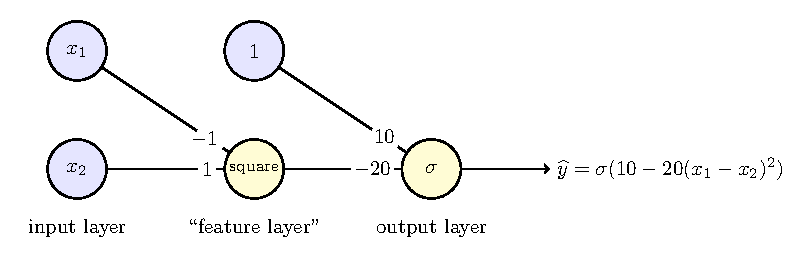
\includegraphics[scale=0.8]{xnor_feature/xnor_feature.pdf}
    \end{figure}

    \begin{center}
        \begin{tabular}{cc|c}
            $x_1$ & $x_2$ & $\widehat{y}$\\\hline
            $0$ & $0$ & $\sigma(10) \approx 1$\\
            $1$ & $0$ & $\sigma(-10) \approx 0$\\
            $0$ & $1$ & $\sigma(-10) \approx 0$\\
            $1$ & $1$ & $\sigma(10) \approx 1$
        \end{tabular}
    \end{center}
\end{frame}

\begin{frame}{What is a neural network?}
    A neural network consists of \textbf{neurons} or \textbf{units}.
    Neurons have \textbf{inputs}, \textbf{outputs}, and \textbf{activations}.
    Connections between these neurons have \textbf{weights}.
    Neurons are organized into \textbf{layers}. \textbf{Hidden layers}
    are sandwiched between an \textbf{input layer} and an \textbf{output layer}.

    Linear regression, logistic regression, and perceptron classification are all
    neural networks, degenerate in the sense that they have no hidden layers.
\end{frame}

\begin{frame}{}
    More formally, a neural network is a function
    \[
        N:\RR^p\lra \RR^q
    \]
    constructed in a particular way.

\end{frame}

\begin{frame}{}
    \begin{align*}
        \text{depth of network (number of layers):\quad}&d\\
        \text{number of neurons in layer $\ell$:\quad}&p_\ell\\
        \text{activation (output) of neuron $k$ in layer $\ell$:\quad}
        & a_k^{[\ell]}\\[1ex]
        \text{bias of neuron $k$ in layer $\ell$:\quad}& b_k^{[\ell]}\\[1ex]
        \text{\parbox{3in}{\raggedleft weight of the connection between neuron $j$\\
        in layer $\ell$ and neuron $i$ in layer $\ell+1$:}\quad}& w^{[\ell]}_{ij}\\
        \text{activation function in layer $\ell$:\quad}&h
    \end{align*}

    \[
        a^{[\ell+1]}_i = h\left(z_i^{[\ell+1]}\right),
        \quad\text{where}\quad
        z_i^{[\ell+1]}=b_i^{[\ell]} + \sum_{j=1}^{p_\ell} w_{ij}^{[\ell]}a_j^{[\ell]}
    \]
\end{frame}

\begin{frame}{}
    \begin{figure}
    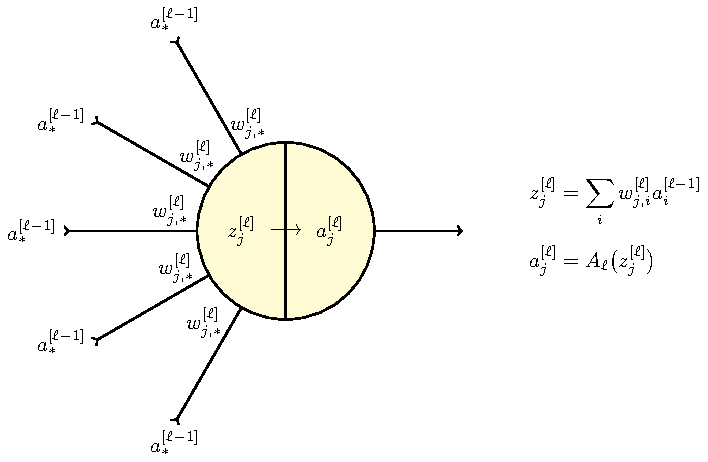
\includegraphics[scale=0.9]{./neuron/neuron.pdf}
    \caption{A hidden or output unit}
    \end{figure}
\end{frame}

\begin{frame}{}
    \begin{figure}
        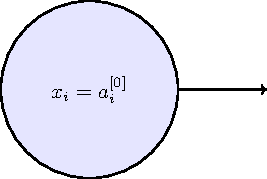
\includegraphics[scale=0.9]{./input/input.pdf}
        \caption{An input unit}
        \end{figure}
    \begin{figure}
    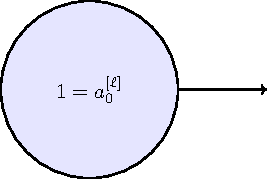
\includegraphics[scale=0.9]{./bias/bias.pdf}
    \caption{A bias unit}
    \end{figure}
\end{frame}

\begin{frame}{}
    \begin{figure}
        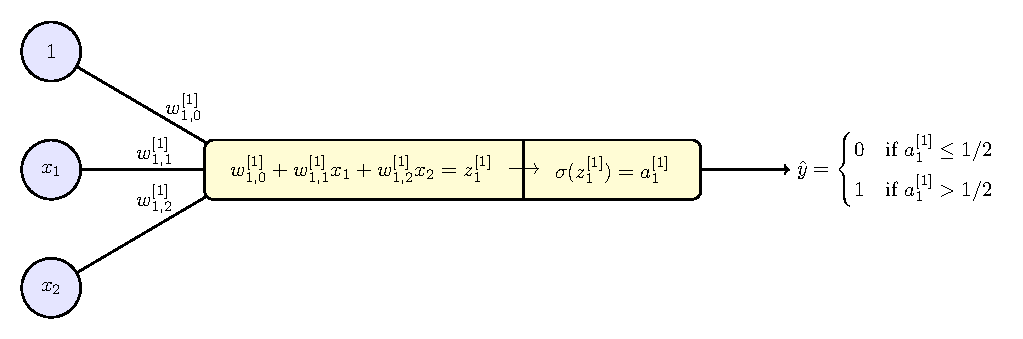
\includegraphics[scale=0.69]{./logistic_regression/logistic_regression.pdf}
        \caption{Logistic regression}
    \end{figure}
\end{frame}

\begin{frame}{}
    \begin{figure}
        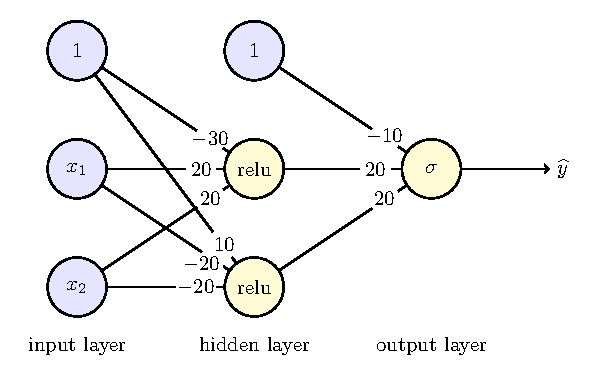
\includegraphics[scale=0.69]{./xnor/xnor.pdf}
        \caption{Learning XNOR}
    \end{figure}

    \begin{center}
    \begin{tabular}{cc|cccc|cc|c}
        $x_1$ & $x_2$ & $z_1^{[1]}$ & $z_2^{[1]}$ & $a_1^{[1]}$ & $a_2^{[1]}$ & $z_1^{[2]}$ & $a_1^{[2]}$ & $\widehat{y}$\\\hline
        $0$ & $0$ & $-30$ & $-10$ & $0$ & $10$ & $190$ & $1.00$ & $1$\\ 
        $0$ & $1$ & $-10$ & $-10$ & $0$ & $0$ & $-10$ & $0.00$ & $0$ \\ 
        $1$ & $0$ & $-10$ & $-10$ & $0$ & $0$ & $-10$ & $0.00$ & $0$\\
        $1$ & $1$ & $-10$ & $-10$ & $10$ & $0$ & $190$ & $1.00$ & $1$
    \end{tabular}
\end{center}
\end{frame}



\end{document}